\chapter{La reproduction sexuée}\label{ch:g8:sexual-reproduction}

Le chant des grenouilles en mai, les \omterm{def:g3:flowers-fruits-seeds:parts}{fleurs} de cerisier en avril, le
brame du cerf en automne, un tournesol qui tourne sa face bien
garnie vers les abeilles~: dans tout le monde vivant, une énorme
\omterm{prop:g3:balanced-diet:jobs}{énergie} est dépensée pour un seul projet --- la génération suivante.
Les années précédentes en ont rassemblé les pièces
(\cref{ch:g4:animal-reproduction},
\cref{ch:g5:flower-to-fruit})~; cette année les assemble en une
seule théorie, et pose la question la plus aiguë~: pourquoi
\emph{deux} parents, au fond~?

\begin{omfigure}
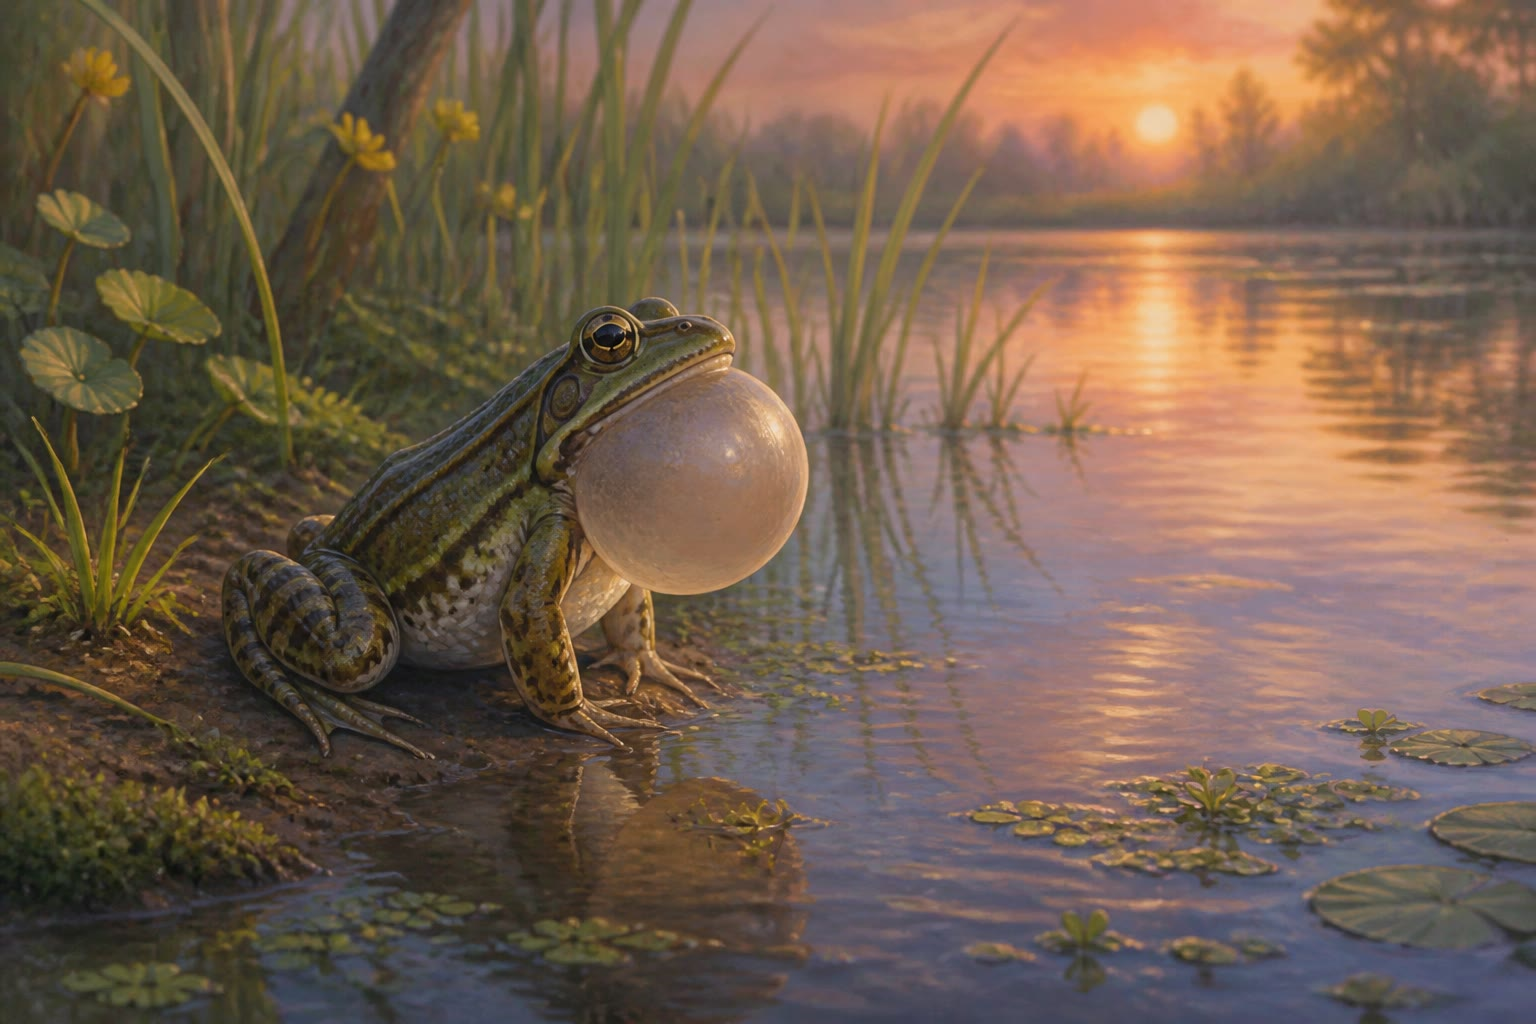
\includegraphics[width=0.6\linewidth]{images/book1/ai/g8-frog-chorus.jpg}

{\small Une énorme \omterm{prop:g3:balanced-diet:jobs}{énergie} pour un seul projet~: le sac vocal gonflé
du \omterm{def:g4:animal-reproduction:sexual}{mâle}, qui convoque la mare pour la rencontre des \omterm{def:g8:sexual-reproduction:gametes}{gamètes}.}
\end{omfigure}

\section{Un seul mécanisme dans tout le monde vivant}

\begin{definition}[Gamètes]\label{def:g8:sexual-reproduction:gametes}
Les \omterm{def:g5:first-look-at-cells:cell}{cellules} reproductrices de
\cref{def:g4:animal-reproduction:sexual} portent le nom général de
\emph{gamètes}\index{gamète}~: le gamète \omterm{def:g4:animal-reproduction:sexual}{mâle} (\omterm{def:g4:animal-reproduction:sexual}{cellule mâle} chez les
\omterm{def:g1:animals-around-us:animal}{animaux}, \omterm{def:g5:first-look-at-cells:cell}{cellule} du grain de \omterm{def:g3:flowers-fruits-seeds:parts}{pollen} chez les \omterm{def:g1:plants-around-us:plant}{plantes} à \omterm{def:g3:flowers-fruits-seeds:parts}{fleurs}) et le
gamète \omterm{def:g4:animal-reproduction:sexual}{femelle} (la \omterm{def:g4:animal-reproduction:sexual}{cellule œuf}, dans l'ovaire ou dans l'ovule). Les
gamètes sont des \omterm{def:g5:first-look-at-cells:cell}{cellules} uniques
(\cref{ch:g5:first-look-at-cells}), et chacun est la moitié d'un
commencement~: seul, un gamète meurt~; réunis, deux font une vie.
\end{definition}

\begin{proposition}[Le noyau invariant]\label{prop:g8:sexual-reproduction:core}
Partout où la \omterm{def:g4:animal-reproduction:sexual}{reproduction sexuée} s'exerce --- poisson ou sapin,
escargot ou humain --- le \omterm{def:g6:cell-unit-of-life:parts}{noyau} est invariable~:
\begin{enumerate}
  \item deux parents produisent des \omterm{def:g8:sexual-reproduction:gametes}{gamètes}, \omterm{def:g4:animal-reproduction:sexual}{mâles} et \omterm{def:g4:animal-reproduction:sexual}{femelles}~;
  \item la \emph{\omterm{def:g5:flower-to-fruit:steps}{fécondation}}~: un \omterm{def:g8:sexual-reproduction:gametes}{gamète} \omterm{def:g4:animal-reproduction:sexual}{mâle} rejoint un \omterm{def:g8:sexual-reproduction:gametes}{gamète}
        \omterm{def:g4:animal-reproduction:sexual}{femelle} et forme une seule \omterm{def:g5:first-look-at-cells:cell}{cellule} nouvelle --- la
        \emph{\omterm{def:g4:animal-reproduction:sexual}{cellule œuf} fécondée}, ou
        \emph{zygote}\index{zygote}~;
  \item le \omterm{prop:g8:sexual-reproduction:core}{zygote} se divise encore et encore
        (\cref{prop:g5:first-look-at-cells:growth}) et bâtit un
        nouvel individu qui porte quelque chose des \emph{deux}
        parents
        (\cref{rem:g4:animal-reproduction:mix}).
\end{enumerate}
Autour de ce \omterm{def:g6:cell-unit-of-life:parts}{noyau}, tout le reste est variation~: où les \omterm{def:g8:sexual-reproduction:gametes}{gamètes} se
rencontrent, combien il y en a, qui s'occupe des jeunes.
\end{proposition}
\admitted

\begin{example}[Les variations, classées]\label{ex:g8:sexual-reproduction:variations}
L'ancienne collection se range proprement sous le \omterm{def:g6:cell-unit-of-life:parts}{noyau}. \omterm{def:g5:flower-to-fruit:steps}{Fécondation}
externe contre \omterm{def:g5:flower-to-fruit:steps}{fécondation} interne
(\cref{prop:g4:animal-reproduction:where})~: le lieu de la
rencontre. \omterm{def:g4:animal-reproduction:ovivivi}{Ovipare} contre \omterm{def:g4:animal-reproduction:ovivivi}{vivipare}
(\cref{def:g4:animal-reproduction:ovivivi})~: le logement du \omterm{prop:g8:sexual-reproduction:core}{zygote}.
Millions de la morue contre petit unique de l'éléphante
(\cref{prop:g4:animal-reproduction:strategies})~: le registre des
nombres. \omterm{def:g5:flower-to-fruit:steps}{Pollinisation} par l'abeille ou par le vent
(\cref{def:g5:flower-to-fruit:steps})~: le service de voyage du
\omterm{def:g8:sexual-reproduction:gametes}{gamète} \omterm{def:g4:animal-reproduction:sexual}{mâle}. Un seul mécanisme, tout un catalogue de réglages.
\end{example}

\begin{remark}[Les plantes suivent le même noyau]\label{rem:g8:sexual-reproduction:plants}
Place \cref{ch:g5:flower-to-fruit} à côté de
\cref{ch:g4:animal-reproduction} et la correspondance est exacte~:
les \omterm{def:g3:flowers-fruits-seeds:parts}{étamines} et le \omterm{def:g3:flowers-fruits-seeds:parts}{pistil} produisent les \omterm{def:g8:sexual-reproduction:gametes}{gamètes}, le tube pollinique
est le couloir de la \omterm{def:g5:flower-to-fruit:steps}{fécondation} interne, la \omterm{def:g2:from-seed-to-plant:seed}{graine} loge l'\omterm{def:g5:human-reproduction:pregnancy}{embryon}
de la \omterm{def:g1:plants-around-us:plant}{plante} avec son casse-croûte emballé
(\cref{def:g2:from-seed-to-plant:seed}). Seule la \omterm{def:g4:plants-without-seeds:vegetative}{reproduction
végétative} (\cref{def:g4:plants-without-seeds:vegetative}) reste à
l'écart --- un seul parent, pas de \omterm{def:g8:sexual-reproduction:gametes}{gamètes}, des copies exactes~: le
contraste qui rend aiguë la question de la section suivante.
\end{remark}

\section{Pourquoi deux parents~?}

\begin{proposition}[La reproduction sexuée brasse les cartes]\label{prop:g8:sexual-reproduction:shuffle}
Les fraisiers copiés par \omterm{ex:g4:plants-without-seeds:runner}{stolons}
(\cref{rem:g4:plants-without-seeds:copy}) montrent ce qu'un seul
parent donne~: de l'identique. Deux parents donnent l'inverse. Comme
chaque \omterm{prop:g8:sexual-reproduction:core}{zygote} combine un \omterm{def:g8:sexual-reproduction:gametes}{gamète} de chaque parent --- et que, comme
un chapitre ultérieur le montrera, deux \omterm{def:g8:sexual-reproduction:gametes}{gamètes} d'un même parent ne
portent jamais tout à fait le même héritage --- la \omterm{def:g4:animal-reproduction:sexual}{reproduction
sexuée} distribue à chaque descendant une \emph{combinaison
nouvelle}. Les frères et sœurs diffèrent~; deux plantules d'une même
cosse ne se ressemblent pas~; la variété à l'intérieur de chaque
\omterm{def:g5:biodiversity:species}{espèce} (\cref{rem:g5:biodiversity:scales}) est largement l'ouvrage
de ce brassage.
\end{proposition}
\admitted

\begin{example}[Les deux paris du verger]\label{ex:g8:sexual-reproduction:bets}
Le verger de \cref{rem:g4:plants-without-seeds:copy} joue les deux
jeux en connaissance de cause. Greffes et \omterm{met:g4:plants-without-seeds:cutting}{boutures}~: un seul parent,
des copies exactes de l'excellent arbre --- et une seule faiblesse
partagée, si bien qu'une maladie qui abat l'un peut les abattre
tous. Pépins~: deux parents, chaque plantule une combinaison
nouvelle --- la plupart quelconques, certaines pires, une rare
meilleure que ses deux parents, et pas deux semblables qu'une
maladie puisse balayer d'un coup. Copier met le présent en banque~;
brasser explore l'avenir.
\end{example}

\begin{remark}[La variété est la réserve de l'espèce]\label{rem:g8:sexual-reproduction:reserve}
Pourquoi le brassage compte au-delà du verger~:
\cref{prop:g5:biodiversity:web} montrait des réseaux qui encaissent
les chocs grâce à la variété des \omterm{def:g5:biodiversity:species}{espèces}~; à l'intérieur d'une
\omterm{def:g5:biodiversity:species}{espèce}, la variété des individus joue le même rôle. Quand les
\omterm{def:g6:exploring-our-environment:conditions}{conditions} tournent --- une nouvelle maladie, un hiver plus dur ---
une \omterm{def:g5:biodiversity:species}{espèce} variée a plus de chances de compter quelqu'un d'adapté
aux nouvelles règles. Ce que cela laisse entrevoir pour l'histoire
de la vie, \cref{ch:g9:how-species-change} le rendra explicite~;
retiens ici seulement que la \omterm{def:g4:animal-reproduction:sexual}{reproduction sexuée} est ce qui garde la
réserve bien garnie.
\end{remark}

\section{Lire la reproduction de n'importe quelle espèce}

\begin{method}[Le dossier de reproduction]\label{met:g8:sexual-reproduction:dossier}
Pour n'importe quelle \omterm{def:g5:biodiversity:species}{espèce}, réunis~:
\begin{enumerate}
  \item les \omterm{def:g8:sexual-reproduction:gametes}{gamètes}~: qui produit lesquels, et où~;
  \item la rencontre~: \omterm{def:g5:flower-to-fruit:steps}{fécondation} externe ou interne, et le
        service de voyage (l'eau, l'\omterm{prop:g4:animal-reproduction:where}{accouplement}, un pollinisateur,
        le vent)~;
  \item le logement~: des \omterm{def:g2:animals-grow-up:born}{œufs} pondus ou des jeunes portés~; avec
        quelles provisions~;
  \item les nombres et les soins~: la position sur la ligne des
        stratégies
        (\cref{prop:g4:animal-reproduction:strategies})~;
  \item la saison~: quand, et calée sur quoi --- la question du
        chapitre suivant.
\end{enumerate}
\end{method}

\begin{example}[Deux dossiers côte à côte]\label{ex:g8:sexual-reproduction:dossiers}
L'épinoche (\cref{exo:g4:animal-reproduction:10})~: \omterm{def:g8:sexual-reproduction:gametes}{gamètes} émis
dans l'eau, \omterm{def:g5:flower-to-fruit:steps}{fécondation} externe, \omterm{def:g2:animals-grow-up:born}{œufs} dans un nid construit, quelques
dizaines, gardés par le père, au printemps. Le cerisier~: \omterm{def:g8:sexual-reproduction:gametes}{gamètes}
dans les \omterm{def:g3:flowers-fruits-seeds:parts}{fleurs}, \omterm{def:g5:flower-to-fruit:steps}{fécondation} interne au bout du tube pollinique,
\omterm{def:g5:human-reproduction:pregnancy}{embryons} logés dans des \omterm{prop:g3:flowers-fruits-seeds:transform}{graines} à l'intérieur des \omterm{prop:g3:flowers-fruits-seeds:transform}{fruits}, par
milliers, pourvus puis abandonnés au service de livraison des
\omterm{prop:g3:sorting-living-things:groups}{oiseaux} (\cref{exo:g6:how-plants-spread:12}), calés sur avril. Même
formulaire, quelle que soit l'\omterm{def:g5:biodiversity:species}{espèce}~: le dossier est la théorie en
usage.
\end{example}

\section{Exercices}

\begin{exercise}[$\star$]\label{exo:g8:sexual-reproduction:1}
Définis \omterm{def:g8:sexual-reproduction:gametes}{gamète} et \omterm{prop:g8:sexual-reproduction:core}{zygote}, et nomme les deux \omterm{def:g8:sexual-reproduction:gametes}{gamètes} chez les \omterm{def:g1:animals-around-us:animal}{animaux}
et chez les \omterm{def:g1:plants-around-us:plant}{plantes} à \omterm{def:g3:flowers-fruits-seeds:parts}{fleurs}.
\end{exercise}

\begin{exercise}[$\star$]\label{exo:g8:sexual-reproduction:2}
Énonce le \omterm{def:g6:cell-unit-of-life:parts}{noyau} invariant en trois étapes.
\end{exercise}

\begin{exercise}[$\star$]\label{exo:g8:sexual-reproduction:3}
Range sous le \omterm{def:g6:cell-unit-of-life:parts}{noyau}~: \omterm{def:g5:flower-to-fruit:steps}{fécondation} externe ou interne, \omterm{def:g4:animal-reproduction:ovivivi}{ovipare} ou
\omterm{def:g4:animal-reproduction:ovivivi}{vivipare}, millions ou petit unique --- que fait varier chacune de
ces paires~?
\end{exercise}

\begin{exercise}[$\star$]\label{exo:g8:sexual-reproduction:4}
Associe les parties de la \omterm{def:g1:plants-around-us:plant}{plante} aux rôles \omterm{def:g1:animals-around-us:animal}{animaux}~: \omterm{def:g3:flowers-fruits-seeds:parts}{étamine},
\omterm{def:g3:flowers-fruits-seeds:parts}{pistil}, tube pollinique, \omterm{def:g2:from-seed-to-plant:seed}{graine}.
\end{exercise}

\begin{exercise}[$\star$]\label{exo:g8:sexual-reproduction:5}
Que donne la reproduction à un seul parent que celle à deux parents
ne donne jamais --- et l'inverse~?
\end{exercise}

\begin{exercise}[$\star$]\label{exo:g8:sexual-reproduction:6}
Pourquoi les frères et sœurs diffèrent-ils, d'après
\cref{prop:g8:sexual-reproduction:shuffle}~?
\end{exercise}

\begin{exercise}[$\star\star$]\label{exo:g8:sexual-reproduction:7}
Explique les deux paris du verger, et dis quand chacun est le bon.
\end{exercise}

\begin{exercise}[$\star\star$]\label{exo:g8:sexual-reproduction:8}
Remplis \cref{met:g8:sexual-reproduction:dossier} pour la grenouille
(toutes les pièces sont dans
\cref{ex:g4:animal-reproduction:song} et
\cref{ex:g2:animals-grow-up:frog}).
\end{exercise}

\begin{exercise}[$\star\star$]\label{exo:g8:sexual-reproduction:9}
Remplis le dossier pour le pissenlit --- avec un avertissement~:
beaucoup de pissenlits font en réalité des \omterm{prop:g3:flowers-fruits-seeds:transform}{graines} sans \omterm{def:g5:flower-to-fruit:steps}{fécondation},
et se clonent par \omterm{prop:g3:flowers-fruits-seeds:transform}{graines}. Quelles rubriques deviennent bizarres, et
que cette anomalie enseigne-t-elle sur les dossiers~?
\end{exercise}

\begin{exercise}[$\star\star$]\label{exo:g8:sexual-reproduction:10}
Un vignoble cultive par \omterm{met:g4:plants-without-seeds:cutting}{boutures} un seul cépage célèbre pendant deux
siècles~; un ravageur arrive, qui raffole précisément de ce cépage.
Raconte de nouveau \cref{ex:g8:sexual-reproduction:bets} comme
l'histoire de ce vignoble.
\end{exercise}

\begin{exercise}[$\star\star$]\label{exo:g8:sexual-reproduction:11}
«~Un \omterm{def:g8:sexual-reproduction:gametes}{gamète} est la moitié d'un commencement.~» Justifie la formule
deux fois~: à partir de l'étape 2 du \omterm{def:g6:cell-unit-of-life:parts}{noyau}, et à partir du brassage.
\end{exercise}

\begin{exercise}[$\star\star\star$]\label{exo:g8:sexual-reproduction:12}
Pourquoi une \omterm{def:g5:biodiversity:species}{espèce} qui sait faire les deux --- le fraisier, avec
ses \omterm{ex:g4:plants-without-seeds:runner}{stolons} \emph{et} ses \omterm{prop:g3:flowers-fruits-seeds:transform}{graines} --- garderait-elle les deux~?
Attribue à chaque mode son service, en te servant de
\cref{rem:g6:how-plants-spread:twospeeds} et de
\cref{rem:g8:sexual-reproduction:reserve}.
\end{exercise}

\section{Problème~: le programme de sélection}

\begin{problem}[{Problème du week-end --- l'année d'une
sélectionneuse, menée d'après la théorie}]\label{pb:g8:sexual-reproduction:1}
Une sélectionneuse veut une nouvelle pomme~: croquante comme la
variété A, résistante à la maladie comme la variété B. Ses outils
sont exactement ceux de ce chapitre.

\medskip\noindent\textbf{Partie I --- Le croisement.}
\begin{enumerate}
  \item Elle prélève au pinceau du \omterm{def:g3:flowers-fruits-seeds:parts}{pollen} sur les \omterm{def:g3:flowers-fruits-seeds:parts}{étamines} de A et
        le dépose sur les \omterm{def:g3:flowers-fruits-seeds:parts}{pistils} de B, puis ensache les \omterm{def:g3:flowers-fruits-seeds:parts}{fleurs}
        contre les abeilles. Nomme le rôle de chaque geste dans le
        \omterm{def:g6:cell-unit-of-life:parts}{noyau} --- et dis pourquoi les sachets comptent
        (\cref{met:g5:flower-to-fruit:diagnose} employait le même
        pinceau).
  \item Que pousse dans le \omterm{prop:g3:flowers-fruits-seeds:transform}{fruit} de B après son passage, et quels
        deux héritages chaque pépin combine-t-il~?
  \item Elle sème trois cents pépins. Pourquoi s'attend-elle à trois
        cents arbres \emph{différents}, d'après
        \cref{prop:g8:sexual-reproduction:shuffle}~?
  \item La plupart des plantules seront quelconques, quelques-unes
        pires que leurs deux parents, une peut-être exactement
        comme il faut. Quel exemple du chapitre prédisait
        exactement cet éventail~?
\end{enumerate}

\medskip\noindent\textbf{Partie II --- Fixer la gagnante.}
\begin{enumerate}[resume]
  \item Huitième année~: un arbre porte des pommes croquantes et
        résistantes. Si elle sème ses pépins, qu'arrive-t-il à la
        combinaison recherchée --- et pourquoi~?
  \item Elle multiplie plutôt la gagnante par greffage --- de
        quelle reproduction s'agit-il, et que garantit-elle~?
  \item Tout son futur verger sera fait des copies de ce seul
        arbre. Nomme le risque qu'elle a accepté, et la formule que
        le chapitre lui donne.
  \item Propose l'assurance habituelle~: que son verger devrait-il
        aussi conserver, et pourquoi cette stratégie fait-elle écho
        à \cref{rem:g8:sexual-reproduction:reserve}~?
\end{enumerate}

\medskip\noindent\textbf{Partie III --- La théorie, mise en
bilan.}
\begin{enumerate}[resume]
  \item Son programme a utilisé les deux paris du verger l'un après
        l'autre. Dis quelle phase a utilisé lequel, et ce que
        chacun lui a apporté.
  \item Un collègue sélectionne des épinoches de la même façon ---
        en choisissant les parents, en élevant les jeunes brassés,
        en gardant les meilleurs. Énumère les rubriques du dossier
        (\cref{met:g8:sexual-reproduction:dossier}) où la pratique
        des \omterm{prop:g3:sorting-living-things:groups}{poissons} diffère de celle des pommes, et les étapes du
        \omterm{def:g6:cell-unit-of-life:parts}{noyau} où elle ne peut pas différer.
  \item La sélectionneuse dit~: «~le sexe propose, la sélection
        dispose --- je ne fais que choisir parmi ce que le brassage
        distribue~». Relie sa devise à la réserve de variété de
        \cref{rem:g8:sexual-reproduction:reserve}.
  \item Une phrase pour conclure~: \emph{à quoi} le programme
        avait-il besoin de la \omterm{def:g4:animal-reproduction:sexual}{reproduction sexuée}, et à quoi de la
        \omterm{def:g4:plants-without-seeds:vegetative}{reproduction végétative}~?
\end{enumerate}
\end{problem}
